\section{Introdução e Justificativa}
\label{sec:int}

Os avanços tecnológicos de sistemas distribuídos estão permitindo que pessoas utilizem de serviços com volumes massivos de dados para aplicações sensíveis a latência. Essa situação é bem favorável a área de jogos massivos, tendo atraído pesquisadores para testar e validar novas abordagens com o objetivo de reduzir a carga e o impacto a latência para o usuário final nesses serviços, resultando em uma melhor experiência aos jogadores da categoria de jogo tratado no presente trabalho\cite{mmo_analytic}.

O mercado de jogos massivos multijogadores de interpretação (\textit{MMORPG}) vem crescendo desde 2012 \cite{new_york_times}, sendo no ano de 2016 um dos mais lucrativos\cite{statista_2016}. A sua projeção para 2018 é que sejam arrecadados mais de 30 bilhões de dólares americanos com esta categoria de jogos \cite{statista_2018}, um aumento de 20\% a mais sobre o ano de 2016.

\textit{Massively Multiplayer Online} ou \textit{MMO} (como são popularmente conhecidos) são os jogos de interpretação multijogador massivos. A principal característica desse estilo de jogo é a comunicação e representação virtual de um mundo fantasia onde cada jogador pode interagir com objetos virtuais compartilhados ou tomar ações sobre outros de jogadores em tempo real, tendo como principais objetivos a resolução de problemas conforme a sua regra de design, o desenvolvimento do personagem e a interação entre os jogadores\cite{video_game_technologies}.

Serviços MMO são utilizados como negócio viável e lucrativo, a qual a experiência de uso do usuário final é um fator crítico para o sucesso. A maioria dos jogos massivos disponíveis no mercado estão implementados sobre uma arquitetura com diversos servidores, onde o desempenho destes servidores influenciam na experiência do usuário final. Modelar um sistema de alto desempenho em torna-se um trabalho essencial para a satisfação do usuário final\cite{1417630}.

\subsection{Ocorrências em serviços massivos}

Uma métrica popular para mensurar o desempenho do jogo é o número de conexões. Em geral, se o servidor caso ultrapasse o limite para qual ele é projetado, diversas ocorrências de experiência com o usuário podem ocorrer. As ocorrências comuns são\cite{1417630}:

\begin{itemize}
  \item \textbf{Longo tempo de resposta aos clientes}: esta ocorrência trás uma qualidade insatisfatória ao usuário ou até mesmo impossibilitando o uso do serviço.
  \item \textbf{Dessincronização com os clientes}: esta ocorrência promove reversão na aplicação, proporcionando desconforto e baixa fluidez do jogo.
  \item \textbf{Problemas internos ao servidor}: esta ocorrência pode estar ligada a diversos outros erros como sobrecarga no banco de dados, gerenciamento lento do espaço ou inconsistências dentro do jogo perante a regra de negócios.
  \item \textbf{Falha de conexão entre o cliente e os microserviços}: promove a inacessibilidade do serviço ao usuário final.
\end{itemize}

Existem algumas causas comuns para essas falhas, sendo alguns dos possíveis problemas conhecidos que podem gerar tais ocorrências\cite{1417630}:

\begin{itemize}
  \item \textbf{Baixo poder computacional do servidor}: poder computacional baixo para a qualidade de experiência do usuário final desejada.
  \item \textbf{Complexidade de algoritmos}: o serviço usa algoritmos de alta complexidade ou até mesmo a regra de negócios que demandem de algoritmos complexos.
  \item \textbf{Limitado pela própria arquitetura}: está limitado a arquitetura que compõe o serviço.
  \item \textbf{Uma arquitetura que não foi planejada ou testada para receber determinada carga}: está limitado diretamente pelo número de conexões.
\end{itemize}

\subsection{Arquiteturas de microserviços}

As ocorrências descritas são resolvidas no segmento de desenvolvimento web utilizando uma arquitetura de microserviços. Entende-se por microserviço as aplicações que executam operações menores, da melhor forma possível, de um macroserviço\cite{stephenclarkewillson2017}. Essas arquiteturas iniciam uma nova linha de desenvolvimento de aplicações preparadas para executar sobre nuvens computacionais, promovendo maior flexibilidade, escalabilidade, gerenciamento e desempenho, sendo a principal escolha de arquitetura de grandes empresas como Amazon, Netflix e LinkedIn\cite{7830692}\cite{7515686}.

A arquitetura ingênua, ou monolítica, é dada por uma única instância agregada com um único banco de dados (relação 1-1). Essa implementação foca somente em criar uma interface global do jogo através desse servidor, recebendo as ações do jogador e retornando o estado de jogo para o cliente. Essa arquitetura é facilmente encontrada em jogos massivos clássicos.

\begin{figure}[H]
  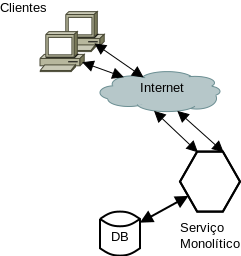
\includegraphics[width=5cm]{arquiteturas/monolitica.png}
  \centering
\end{figure}

A arquitetura de múltiplos canais\cite{1417630} é uma arquitetura de microserviços que baseia-se na divisão dos clientes em instâncias de jogos diferentes, utilizando a mesma base de de dados (relação n-1). Se faz necessário um gerenciador de contas, para impedir multiplas conexões em canais diferentes da mesma conta.

\begin{figure}[H]
  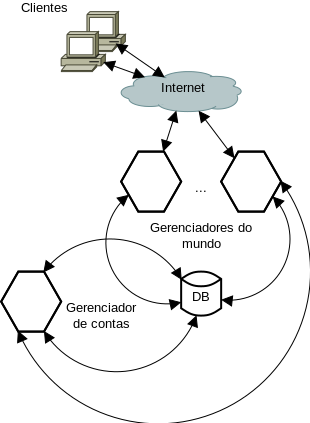
\includegraphics[width=5cm]{arquiteturas/multiplos_canais.png}
  \centering
\end{figure}

A arquitetura baseada em regiões\cite{albion_online_unite} basea-se na distribuição uniforme dos jogadores no mundo virtual, visando distribuir os jogadores dentre os multiplos serviços por região. Os bancos de dados foram retirados para facilitar a visualização.

\begin{figure}[H]
  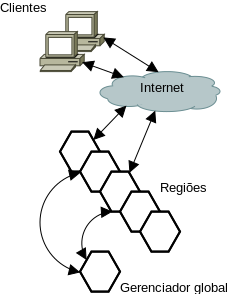
\includegraphics[width=5cm]{arquiteturas/regioes.png}
  \centering
\end{figure}

A arquitetura baseada em serviços\cite{stephenclarkewillson2017} aborda o jogo como um único servidor monolítico, separando as suas funcionalidades em microserviços. Esta arquitetura arrisca tempo de resposta para obter o máximo de conexões no macroserviço. Também utiliza a abordagem de separação das regiões focando na distribuição uniforme dos jogadores no mundo virtual. Os bancos de dados foram retirados para facilitar a visualização.

\begin{figure}[H]
  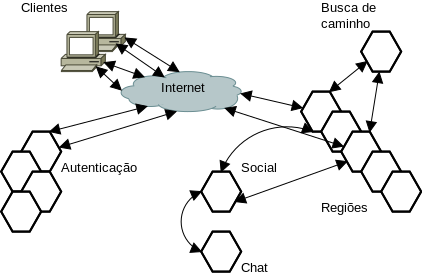
\includegraphics[width=8cm]{arquiteturas/servicos.png}
  \centering
\end{figure}

\subsection{Justificativa}

A proposta de otimização das análises realizadas sobre as arquiteturas de microserviços para jogos massivos focada ao gerenciamento de mundos virtuais proposta pela literatura traz impacto direto a melhoria da qualidade de experiência ao usuário final e maior margem de lucro\cite{1417630}, por sua vez, proporcionando soluções com melhor garantia de sucesso sobre outras arquiteturas problemáticas.
